\documentclass[11pt, a4paper]{toptesi}

\usepackage[utf8]{inputenc} %utf8
\usepackage[english]{babel}
\usepackage[T1]{fontenc}
\usepackage{blindtext}
\usepackage{graphicx,wrapfig}
\usepackage{booktabs}
\usepackage{lmodern}
\usepackage{varioref}
\usepackage{url}
\usepackage{array}
\usepackage{verbatim} 
\usepackage{subfig}
\usepackage{tabularx}
\usepackage{amsmath}
\usepackage{amsfonts}
\usepackage{float}
\usepackage{amssymb}
\usepackage{multicol}
\usepackage{multirow}
\usepackage{listings}
\usepackage{algorithm}
\usepackage{algorithmic}
\usepackage{amsmath}
\usepackage{hyperref}
\usepackage{minted}
\usepackage{fancyhdr}
\frenchspacing
\pagestyle{fancy}
\begin{document}

\paragraph{Laboratory report (Features and Panoramic Image) - Luca Dolci 1234008}
The program provides the class \mintinline{R}{PanoramicImage} which compute the 
panoramic image by merging together some input images. The public
interface is composed by the \mintinline{R}{loadImages()} method, which
harvest the images from a given directory, and by the
\mintinline{R}{elaborate()} method which performs the computation in steps:
\begin{enumerate}
    \item Project every single image in a cylindrical surface. The FOV parameter
        is different for each dataset provided.
    \item Extract the feature from each different image. This is done using 
        SIFT features (with $l_2$ norm). In this step the descriptors for each
        keypoints are also computed. The methods \mintinline{R}{detect()} and
        \mintinline{R}{compute()} of the class \mintinline{R}{SIFT} are used for
        the keypoints and the descriptors, respectively. The results after this
        step is the seguent:
         \begin{center}
             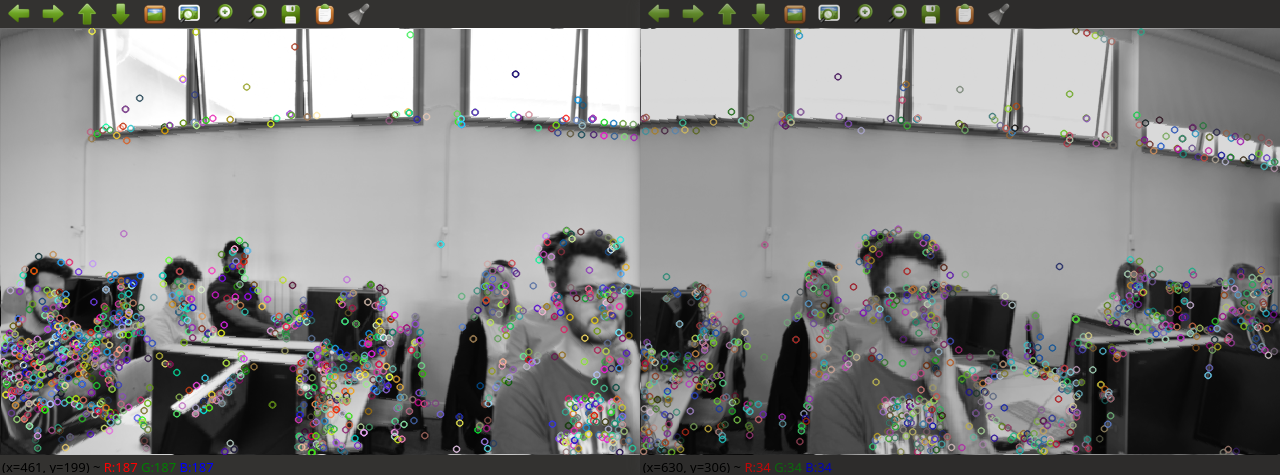
\includegraphics[width=0.85\textwidth]{features.png}
        \end{center}
        In this two images 1266 and 992 feaures are detected for the first and
        second image.
    \item Features matching. Performed using the brute force method (mehtod
        \mintinline{R}{match()} of the class BGMatcher, which requires two set
        of descriptors computed in previous step), the result is a set of istances of
        the DMatch class. Each istance provides the distance of the two
        keypoints and the index of the matched keypoints, one for the left image
        and one for the right image. The result of this step on the first two
        images is the seguent:
         \begin{center}
             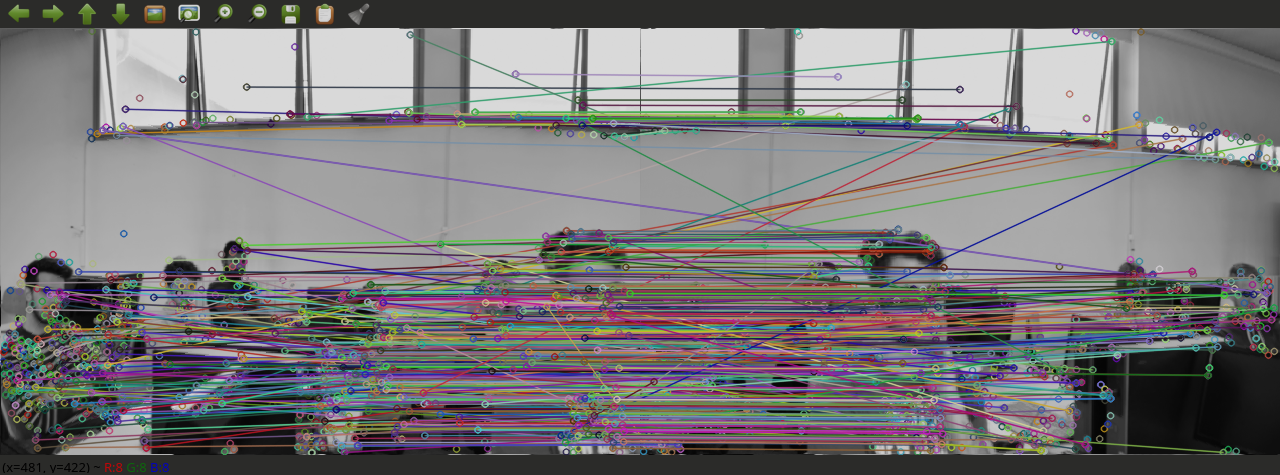
\includegraphics[width=0.85\textwidth]{match1.png}
         \end{center}
         457 matches are found.
    \item Matches refinement. This step has two substeps:
        \begin{enumerate}
            \item Discard matches based on distance. The matches for each pair
                of images are discarded if their distance is less or equal than
                the minmum times the ratio, a crucial parameter that the user
                can set at the beginning of the computation. This can change the
                alignment (a future step). A low value can cause a poor
                alignment because lots of matches will be discarded and the
                alignment will be based on few matches, on the other hands, with
                a too high value some fake matches can remain, which can cause
                disaligment.
            \item Discard matches based on homography. The matches for each pair
                of images are discarded if they are labeled as 'outilers' by the
                RANSAC algorithm. This actually helps a lot, discarding matches
                with different 'slope' (see figure below) from the rest of the
                matches.
        \end{enumerate}
        The result, with ratio equal to 10, is the seguent:
         \begin{center}
             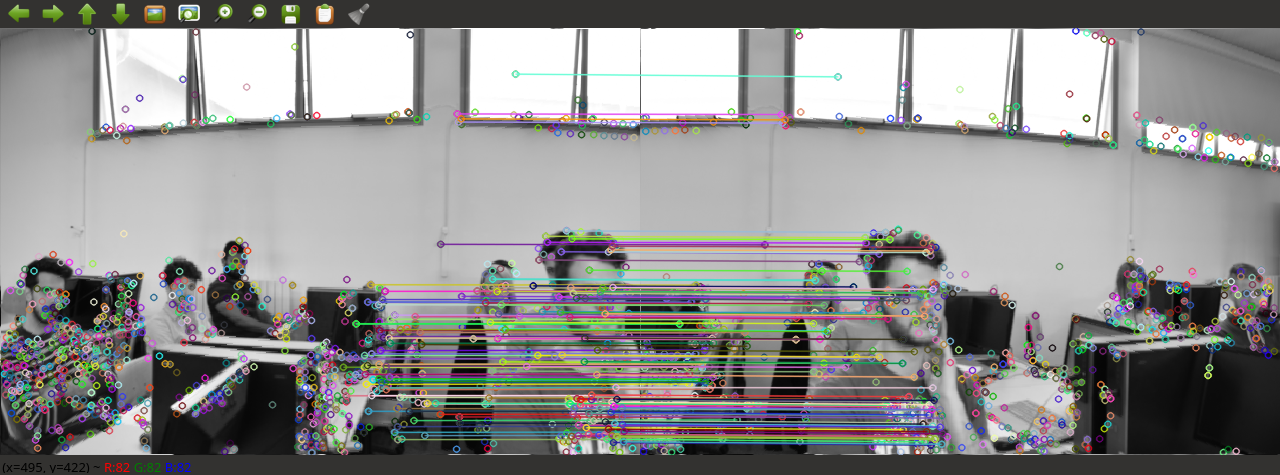
\includegraphics[width=0.85\textwidth]{match2.png}
         \end{center}
         The remaining  matches are 164. With ratio equals to two ony 9 matches
         remains.
    \item Alignment. For each image and for each matches set (one on the left
        and one on the right) the mean position of the keypoints are computed.
        This represent the translation on the x and y axis, which are
        indipendet:
        \begin{itemize}
            \item on the x axis: each image is cropped such that the left margin
                match the x coordinate of the mean position of keypoints matched
                with the left image, the same on the right. If this coordinates
                overlaps, the image is discarded.
            \item on the y axis: each image is translated with respect to the
                posion on the first image, computing the local translation with
                the left image (difference between the y coordinate in the
                positions of the mathced keypoints) and performing the
                translation using an affine transformation and a transformation
                matrix.
        \end{itemize}
        Finally the whole image can be cropped in order to avoid black strips.
        The final result is the seguent:
         \begin{center}
             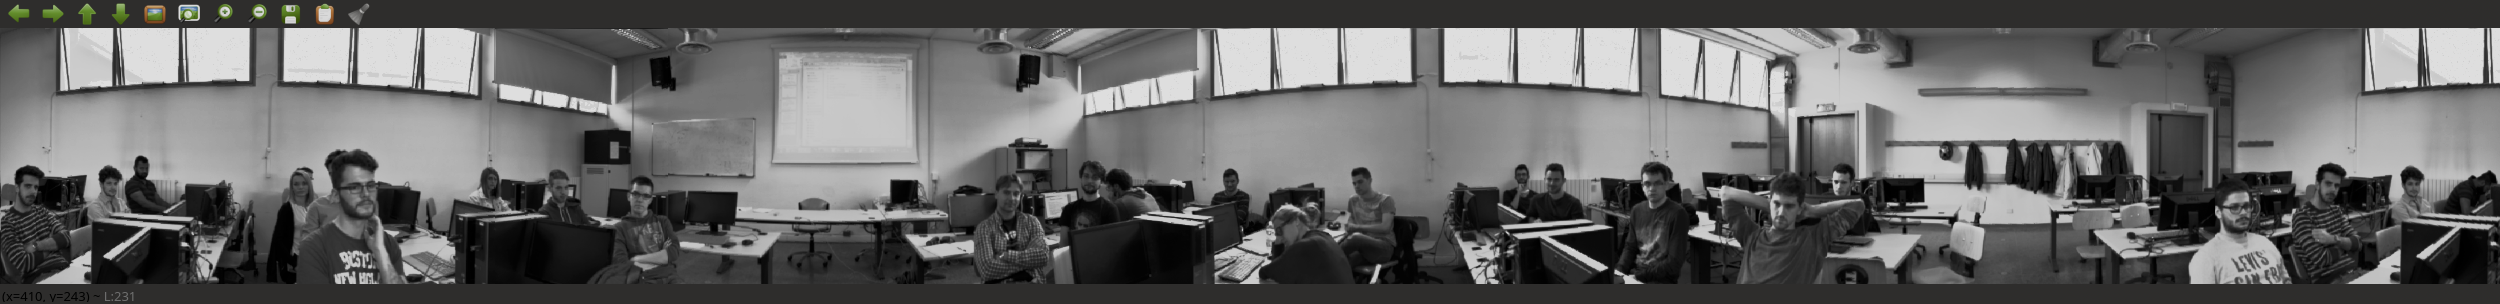
\includegraphics[width=0.9\textwidth]{panoramic.png}
         \end{center}


\end{enumerate}       
\end{document}
